\documentclass[a4paper,11pt]{report}
\usepackage[utf8]{inputenc}
\usepackage[T1]{fontenc}
\usepackage[francais]{babel}
\usepackage{graphicx}
\usepackage{geometry}



\title{Logiciels de sauvegarde}
\author{Edgar RODRÍGUEZ}


\begin{document}
\maketitle

\section{Areca Backup}
\subsection{Principales caractéristiques}
\begin{itemize}
  \item Archives de compression en format Zip et Zip64.
  \item Archives de cryptage (AES128 et algorithmes de chiffrement AES 256).
  \item Stockage sur disque dur local, lecteur réseau, clé USB, FTP, FTPS (implicite et explicite avec SSL / TLS) ou un serveur SFTP.
  \item Filtres de fichier : par extension, répertoire, expression régulière, taille, date, statut, avec AND / OR /NOT logique.
  \item Sauvegarde Incrémentielle, différentielle et sauvegarde complète.
  \item Archives et fusions : Permet fusionner les archives contigus dans une archive unique pour économiser l'espace de stockage.
  \item Sauvegarde à partir d'une date donnée : Permet de récupérer des archives à partir d'une date spécifique.
  \item Mécanisme de transaction : tous les processus critiques, telles que les sauvegardes ou fusions sont transactionnels (commit rollback). Cela garantit l'intégrité des sauvegardes.
  \item Rapports de sauvegarde : Areca génère des rapports de sauvegarde qui peuvent être envoyés par email.
  \item Progammation de scripts de sauvegarde : Areca peut lancer des scripts shell après la sauvegarde.
  \item Les permissions des fichiers, liens symboliques et les pipes nommés peuvent être stockés et récupérés (Linux uniquement).
\end{itemize}

\subsection {Modes de stockage}
Areca peut gérer de multiples modes de stockage:
\begin{itemize}
  \item Standard: C'est le mode par défaut, une nouvelle archive sera créée pour chaque sauvegarde. Tous les fichiers nouveaux ou modifiés depuis la dernière sauvegarde seront stockés dans cette archive.
  \item Delta: Une nouvelle archive sera créée pour chaque sauvegarde. Tous les *parties* modifiées de fichiers depuis la dernière sauvegarde seront stockés dans cette archive. Ce mode est particulièrement utile pour la manipulation des fichiers volumineux. (Areca utilise un algorithme qui est similaire à rsync pour détecter et gérer les parties modifiées des fichiers).
  \item Image: Une archive unique sera créé et mis à jour à chaque sauvegarde.
\end{itemize}

\subsection {types de sauvegarde}
Areca peut gérer les types de sauvegardes suivants:
\begin{itemize}
  \item Sauvegarde complète: Lors d'une sauvegarde complète est effectuée, tous les fichiers sont stockés dans une archive (même s'ils ont été modifiées ou non).
  \item Sauvegarde incrémentale: Quand une sauvegarde incrémentale est réalisée, seuls les fichiers qui ont été modifiés depuis la dernière sauvegarde sont stockés dans l'archive.
  \item La sauvegarde différentielle: Lors d'une sauvegarde differentiel est effectuée, seuls les fichiers qui ont été modifiés depuis la dernière sauvegarde complète sont stockés dans l'archive.
\end{itemize}

Areca utilise la taille du fichier et date de dernière modification pour détecter les fichiers modifiés, si un de ces attributs est modifié (quelle que soit sa valeur), le fichier est marqué comme modifié. Cela permet une détection rapide des fichiers modifiés.

\subsection {Target}

Une tâche de sauvegarde est appelée «target» dans la terminologie de Areca. Il définit les fichiers qui seront stockés (sources), où ils seront stockés (destination) la façon dont ils seront stockés (si elles seront compressées, cryptées, etc.).
Les «targets» peuvent être organisés en «targets groups».

\begin{figure} [h]
\begin {center}
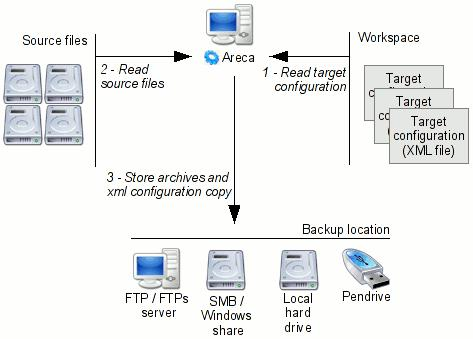
\includegraphics[width=0.5\textwidth]{areca_backup.jpg}
\caption{Exemple d'usage d'Areca Backup}
\end {center}
\end{figure}


\section{Bacula}
Bacula est un ensemble de programmes qui permet de gérer des sauvegardes, restaurations ou vérifications de données d'un ordinateur sur un réseau hétérogène.
\subsection{Principales caractéristiques}
\begin{itemize}
  \item Il utilise une base de données relationnelle motorisée par MySQL, PostgreSQL ou SQLite.
  \item Crée des signatures SHA-1 (ou MD5) pour chaque fichier sauvegardé.
  \item Permet le chiffrement des données et des commandes transitant sur le réseau et peut sauvegarder des fichiers de plus de 2 Go.
  \item Capable de gérer les robots changeurs de bandes.
  \item Peut exécuter des scripts avant et après de chaque travail.
\end{itemize}

\subsection{Services de Bacula}
\begin{itemize}
  \item Le service \textbf{Bacula Director} est le programme qui supervise toutes les opérations de sauvegarde, restauration, vérification et archivage. L'administrateur système utilise le Bacula Director pour planifier les sauvegardes et restaurer les fichiers.
  \item Le service \textbf{Bacula Console} est le programme qui permet à l'administrateur ou à l'utilisateur de communiquer avec le Bacula Director. Actuellement, le service Bacula Console est disponible en trois versions. La première et la plus simple est d'exécuter le programme Console dans une fenêtre shell (i.e. interface TTY). La seconde version est une interface graphique GNOME. La troisième version est une interface graphique wxWidgets qui permet de sélectionner interactivement les fichiers à restaurer. Elle intègre la plupart des fonctionnalités de la console shell, permet la complétion automatique avec la touche tabulation, et fournit une aide instantanée relative à la commande tapée.
  \item Le service \textbf{Bacula File} (ou programme client) est le programme installé sur la machine à sauvegarder. Il est spécifique au système sur lequel il est exécuté et a la charge de fournir les attributs des fichiers et les données requis par le Director. Les Services File sont aussi chargés de la partie dépendant du système de fichiers lors de la restauration des attributs de fichiers et des données. Ce programme est exécuté en tant que service sur la machine à sauvegarder. En plus du File Daemon pour Unix/Linux, il existe un File Daemon pour Windows (usuellement distribué au format binaire). Le File Daemon Windows fonctionne sur toutes les versions actuelles de Windows (NT, 2000, XP, 2003 et peut-être aussi 98 et Me).
  \item Le service \textbf{Bacula Storage} est le programme qui transfère les données et les attributs de fichiers aux média physiques ou aux volumes et les restitue lors de restaurations. En d'autres termes, Le storage Daemon est responsable des opérations de lecture et d'écriture sur les cartouches (ou autres média de stockage, comme par exemple des fichiers).
  \item Les services \textbf{Catalogue} ont pour tâche de maintenir à jour la base de données des index de fichiers et volumes pour tous les fichiers sauvegardés. Les services Catalogue permettent à l'administrateur système ou à l'utilisateur de localiser rapidement et restaurer n'importe quel fichier. Les services Catalogue de Bacula le placent dans une catégorie différente de programmes tels que tar et bru, puisque le catalogue Bacula maintient un enregistrement de chaque volume utilisé, chaque job exécuté et chaque fichier sauvegardé ce qui permet des restaurations et une gestion de volumes efficaces.
\end{itemize}

\begin{figure} [h]
\begin {center}
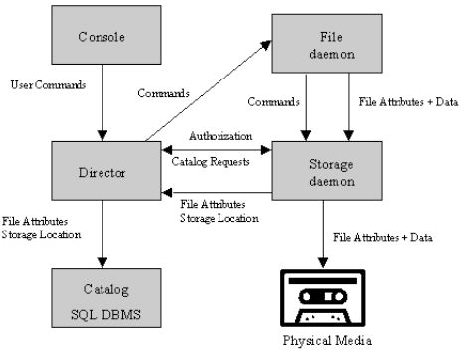
\includegraphics[width=0.5\textwidth]{bacula.png}
\caption{Interactions entre les services Bacula.}
\end {center}
\end{figure}




\section{BackupPC}
\subsection{Caractéristiques}
\begin{itemize}
  \item Support des sauvegardes complètes, incrémentielles ou partielles (possibilité de reprise sur erreur).
  \item Capable de sauvegarder sur disque un ensemble de postes clients et de serveurs, sous Unix, Linux, Windows ou Mac OSX. 
  \item Les protocoles utilisables pour les transferts sont : SMB, tar over SSH/rsh/nfs, et rsync. 
  \item Il ne nécessite l'installation d'aucun logiciel client sur les machines à sauvegarder.
  \item Il possède une interface web pour lancer des sauvegardes ou restaurer des fichiers. 
  \item Il est également possible de sauvegarder des bases de données via un script shell lancé avant la sauvegarde.
  \item Remontées d'alertes par e-mail pour chaque utilisateur : Ordinateur non sauvegardé depuis trop longtemps (car non connecté au réseau, par exemple), ou erreurs dans la sauvegarde.
  \item Support des sauvegardes de machines portables, machines connectées de façon intermittente, ou avec adresses IP variables (exemple : DHCP dynamique).
  \item Compression des fichiers sur le serveur de sauvegarde
élimine les redondances entre fichiers identiques (déduplication au niveau fichier) : gain d'espace sur le serveur.
  \item Possibilité pour les utilisateurs de déclencher manuellement une sauvegarde complète ou incrémentale (en dehors du calendrier calculé par le serveur), possibilité de planifier manuellement une sauvegarde à rythme régulier.
  \item Possibilité pour les utilisateurs de modifier certains paramètres de sauvegardes (selon restrictions faites par l'administrateur)
  \item Authentification des utilisateurs (accès à l'interface web) via HTTP ou LDAP.
\end{itemize}

\subsection{Stockage}
\begin{itemize}
  \item Stockage des données au format GZIP.
  \item Possibilité d'extraction des données au format TAR et GZIP.
  \item Possibilité d'archivage vers supports amovibles (ex. bandes) au format TAR.
  \item Utilise les protocoles standards SSH, RSYNC, NFS, SMB, FTP pour effectuer la sauvegarde des machines.
\end{itemize}


\section{luckyBackup}
\subsection{Caractéristiques}
\begin{itemize}
  \item Simple avec toute la puissance de rsync dans une interface conviviale.
  \item Possibilité de créer des profils de sauvegarde différents, ce qui nous donne une grande flexibilité dans l'organisation des tâches de sauvegarde.
  \item Planification de l'exécution de profils déjà créés par cronjobs est pris en charge.
  \item Sécurité: Toujours vérifier le dossier de destination, voir s'il ya invalide ou vide.
  \item Possibilité de synchroniser des dossiers, en gardant les fichiers les plus récents des deux.
  \item Possibilité d'exclure les données à partir d'une tâche.
  \item Possibilité d'inclure uniquement les données spécifiques.
  \item Exécuter des commandes avant et après une travail.
  \item Le mode simulation.
\end{itemize}




\section{Amanda}
\subsection{Principales caractéristiques}
\begin{itemize}
  \item Il est basé sur des outils standards (dump, restore, tar, etc.).
  \item Son architecture modulaire répartit, les tâches sur des machines périphériques. Par exemple, le serveur peut ne pas accueillir de dérouleur.
  \item Architecture un client/serveur : Permet la possibilité de réaliser des copies de systèmes physiquement éloignés mais branchés sur le même réseau et génère un environnement facilement escalable.
  \item Une Sécurité : Les communications peuvent être protégés en utilisant OpenSSH ou des algorithmes de chiffré.
  \item Cache dans un disque : Amanda stocke les copies dans un disque pour éviter des pertes de données et pour améliorer la vitesse d'enregistrement.
  \item Il implémente une gestion des bandes simple et efficace : on ne peut effacer une bande par erreur, et il existe des outils de recherche de fichier dans toute la collection de support.
  \item Interface générique des changeurs de bandes, donc, non seulement on peut utiliser des dérouleurs différents, mais aussi des robots différents.
  \item Ajuste l’ordonnancement par des règles d’optimisation.
  \item Intégre des outils de rapport, hautement configurables et modifiables.
  \item Autorise l’inclusion de tout module que l’on désire.
  \item Peut encrypter ou compresser tant les communications avec les agents de sauvegarde, que les supports eux-mêmes.

\end{itemize}

\begin{figure} [h]
\begin {center}
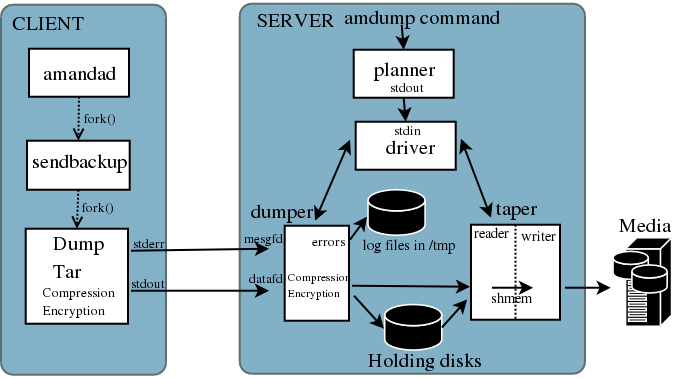
\includegraphics[width=0.5\textwidth]{amanda.png}
\caption{\textbf{beginamandad:} Le processus du client qui exécution des requêtes du serveur invoquant d'autres commandes.
\textbf{amdump:} commande qui démarre le processus de copie sur le serveur en fonction des paramètres définis par l'utilisateur.
\textbf{Media:} Support dans lequel est stocké la sauvegarde.}
\end {center}
\end{figure}








\end{document} 
